% !TeX root = ../main.tex

\chapter{二值友好网络结构设计}

\section{概述}

神经网络二值化可以节省大量的存储资源和计算资源,有利于基于神经网络的算法部署到资源受限设置,近年来受到了学术界和工业界越来越多的关注。神经网络二值化本质是激活值和权重的二值化,将激活值和权重从32为量化为1位,可以将卷积计算中的乘加操作用位运算代替,加快网络的推理速度,然后1位的激活值和权重的表示能力相比32位大大降低,导致二值神经网络的性能与同结构浮点网络相比相差较多。与8位定点量化不同,神经网络二值化过程中激活值和权重的剧烈改变会大幅度改变网络拟合的函数族。因此适合于浮点网络的网络结构设计可能不再适合于二值网络,不适合浮点网络的网络结构可能在二值网络中发挥巨大作用。

为了提高二值神经网络的性能,使其达到浮点网络的精度水平,需要针对二值神经网络的特点专门设计二值友好结构。Bi-real Net\cite{birealnet}为每个卷积模块插入残差连接,最大程度地保留了浮点特征的信息并减小梯度方向传播过程中的误差累积,该设计被后续大多数二值神经网络所使用。WRPN\cite{wrpn}和MeliusNet\cite{meliusnet}通过增加通道数改变二值网络结构,同样提升了二值网络的信息处理能力。XNOR-Net\cite{xnornet}、XNOR-Net++\cite{xnornet++}、ReActNet\cite{reactnet}等二值网络通过引入逐元素计算的缩放因子或激活函数提高二值网络的特征表达能力。

本文进一步探究了神经网络基本组成成分对二值神经网络的影响。从XNOR-Net\cite{xnornet}开始,二值神经网络普遍采用归一化层\ -\ 二值函数层\ -\ 卷积层\ -\ 激活层的模块网络层排布顺序,其基本思想是通过归一化层调整浮点特征的分布,使浮点特征的均值在0附近,这时使用阈值为0的符号函数作为二值函数,可以将浮点特征分成元素数量近似相等的两部分。本文探究了浮点特征分布对二值卷积的影响,提出了与XNOR-Net不同的观点,本文认为二值特征中1和-1的个数均衡不能使二值特征的信息量更高,1和-1的个数的比例需要网络自行调整,并以此为根据设计了新的网络层排布顺序。二值神经的特征提取能力受到二值卷积的限制,因此在二值网络中,浮点运算发挥着重要的作用。二值网络中的浮点运算不仅可以调整特征的分布,还起到辅助卷积进行特征提取的作用。本文探究了浮点运算在二值网络中的作用,提出了专用于二值网络的逐元素浮点运算模块,以极低的计算量代价换取较多的性能提升。

本章的主要贡献如下:

(1)本文分析了二值网络中二值卷积的特点,提出二值函数层\ -\ 卷积层\ -\ 激活层\ -\ 归一化层的全新网络层结构顺序,相比其他二值网络中使用的传统顺序更有利于网络的特征提取。

(2)本文探究了浮点运算在二值网络中的作用,提出全新的分段线性缩放模块,将该激活函数插入二值网络主干可以大幅提高二值网络的推理精度。

\section{二值友好的网络模块设计}

现代卷积神经网络结构基本都由模块(block)组成,模块指神经网络中重复使用的一组网络层的连接结构,一般包括卷积层、归一化层、激活层等网络层和残差连接,经典的ResNet网络的模块如图 \ref{fig:res_block} 所示,1个残差连接中包括了2个卷积层和1个ReLU非线性激活层,归一化层紧跟在卷积层后面,这是在网络特征使用浮点数表示取值范围极大的条件下的设计。二值网络由于其数值表示的特征性而不适合使用这种设计,Bi-real Net\cite{birealnet}首先提出在每个二值卷积外都使用一条残差连接,其模块设计如图 \ref{fig:bireal_block} 所示。其中Sign表示二值函数层,该网络去掉了ReLU非线性激活层,仅使用符号函数实现网络的非线性功能。本文沿用Bi-real Net\cite{birealnet}中的单卷积网络模块结构,分析了现有二值网络模块设计的不足,探究了有利于二值网络的微浮点计算操作,提出了更适合二值网络的模块设计。

\begin{figure}[htb]
  \vspace{6pt}
  \centering
  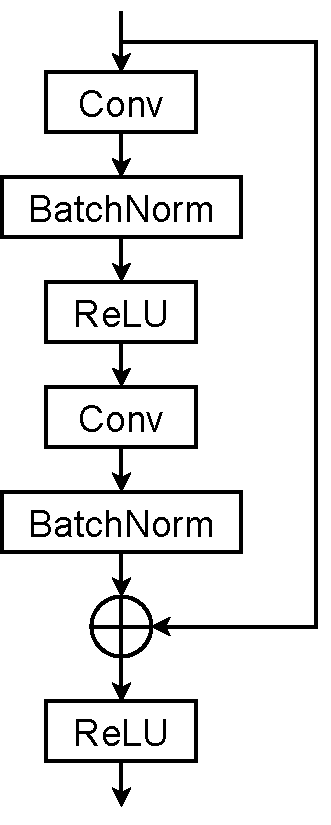
\includegraphics[width=0.22\textwidth]{res_block.pdf}
  \caption{ResNet网络模块结构示意图}
  \label{fig:res_block}
\end{figure}

\begin{figure}[htb]
  \vspace{6pt}
  \centering
  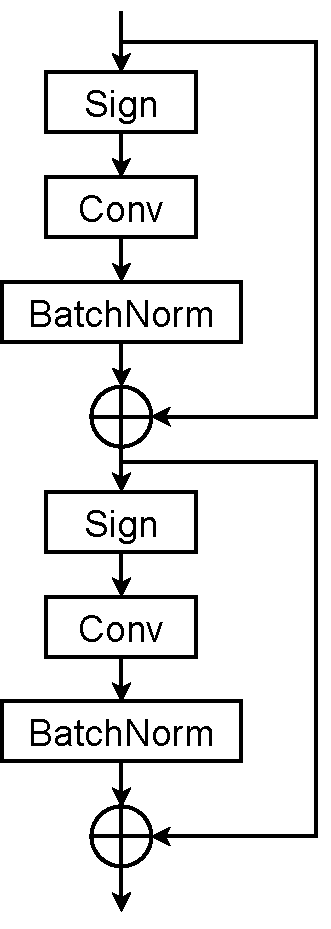
\includegraphics[width=0.22\textwidth]{bireal_block.pdf}
  \caption{Bi-real Net网络模块结构示意图}
  \label{fig:bireal_block}
\end{figure}

\subsection{模块内网络层选择与顺序设计}

二值网络激活值的分布会影响网络的性能,XNOR-Net\cite{xnornet}和IR-Net\cite{irnet}提出激活值均匀分布在原点两侧时最有利于二值化过程的信息保存,此时二值特征图的信息熵最大,本文则提出不同的观点。卷积操作是模式匹配操作,其输出结果是模式匹配的响应强度,因此网络前向传递时的特征表示了每层网络解析后的响应强度,我们应更关注响应强度大的部分。将浮点特征二值化为二值特征时,如果限制激活值以原点为对称轴左右均匀分布,就会使较大的激活值和接近0的激活值被二值化为相同的结果,这会抹平强响应与弱响应之间的区别。因此本文认为不应该强制将浮点特征图的均值调整到0附近,即不需要再卷积层前添加归一化层。

浮点网络中通常使用ReLU函数作为激活函数,为网络提供非线性拟合能力。ReLU函数定义如公式 \eqref{eq:relu} 所示,该函数仅保留正的激活值,舍弃掉负的激活值。

\begin{equation}
  \label{eq:relu}
  f(x) =
  \begin{cases}
    x & if \ x > 0 \\
    0 & if \ x \leq 0
  \end{cases}
\end{equation}

在二值网络中,激活值被量化为-1和1,正负激活值都应该被保留,因此二值网络一般不使用ReLU函数作为激活函数。一些研究认为作为二值函数的符号函数已经提供了非线性能力,不需要额外的非线性激活函数,本文则认为激活函数不仅提供非线性拟合能力,还可以补充二值卷积的特征提取能力,因此需要在网络模块内添加激活函数。本文使用PReLU作为模块内的激活函数,PReLU函数定义如公式 \eqref{eq:prelu} 所示:

\begin{equation}
  \label{eq:prelu}
  f(x) =
  \begin{cases}
    x & if \ x > 0 \\
    \beta x & if \ x \leq 0
  \end{cases}
\end{equation}
其中$\beta$是可学习参数,和权重参数一样在网络训练过程中自适应优化,训练开始前一般将$\beta$参数的初始值设置为0.25,使该函数具有一定的非线性性,训练过程中$\beta$可以被优化为正值和负值在内的任意值。

由于PReLU激活函数具有一个逐元素浮点计算,因此可以作为二值卷积特征提取的补充,为了避免归一化层对PReLU层解析卷积结果的干扰,本文将PReLU函数层放置在卷积层后面,归一化层前面。本文提出的网络模块结构如图 \ref{fig:mfnet_block} 所示,4.4节的实验测试了不同网络层排布顺序的网络精度,本文提出的网络层排布精度最高,验证了激活函数的特征提取作用。

\begin{figure}[htb]
  \vspace{6pt}
  \centering
  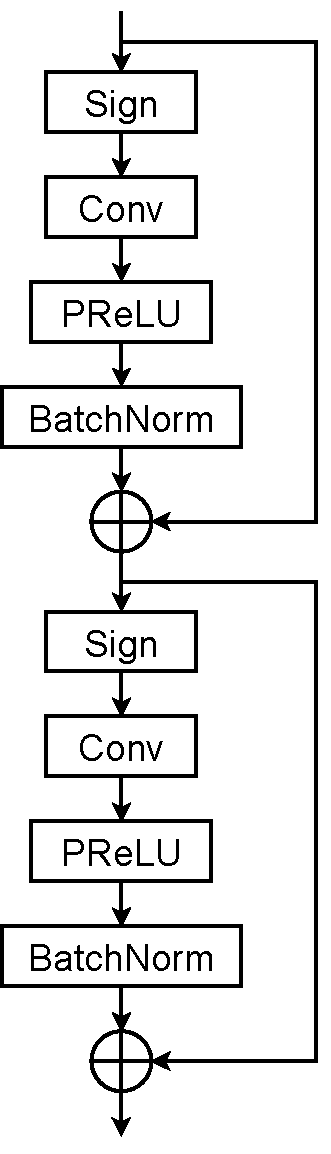
\includegraphics[width=0.22\textwidth]{mfnet_block.pdf}
  \caption{本文提出的网络模块结构示意图}
  \label{fig:mfnet_block}
\end{figure}

\subsection{面向二值网络的模块间激活函数}

二值神经网络使用二值卷积进行特征提取,二值卷积中进行的1位乘加运算可以用同或运算和位计数运算代替,从而提高运算速度,但是1位权重仅有-1和1两种取值,特征提取能力极其有限,限制了二值网络的性能。XNOR-Net\cite{xnornet}等网络引入了缩放因子,本质上增加了逐元素的浮点乘法,实验表明这些极低计算量的浮点乘法可以使二值网络的性能大幅提升。

% ReActNet\cite{reactnet}提出RPReLU激活函数,该函数定义如公式 \eqref{eq:rprelu} 所示:

% \begin{equation}
%   \label{eq:rprelu}
%   f(x) =
%   \begin{cases}
%     x - \gamma + \zeta  & if \ x > \gamma  \\
%     \beta (x - \gamma) + \zeta  & if \ x \leq \gamma 
%   \end{cases}
% \end{equation}
% 其中$\beta$、$\gamma$和$\eta$都是可学习参数,ReActNet将该激活函数插入网络模块之间,用来调整浮点特征图的分布。

为了提升二值网络的性能,本文设计了用于二值网络的分段线性缩放激活函数,该函数定义如公式 \eqref{eq:pw} 所示:

\begin{equation}
  \label{eq:pw}
  f(x) =
  \begin{cases}
    \beta_1 x & if \ x > 0 \\
    \beta_2 x & if \ x \leq 0
  \end{cases}
\end{equation}
其中$\beta_1$和$\beta_2$是两个独立的可学习参数,分别用于控制正数特征和负数特征,与缩放因子相比,分段线性缩放同样逐元素进行一次逐元素浮点乘法操作,但是增加了基于特征取值选择乘法系数的能力,这种选择能力在几乎不增加计算量的前提下使该激活函数具有一定的非线性性。

\begin{figure}[htb]
  \vspace{6pt}
  \centering
  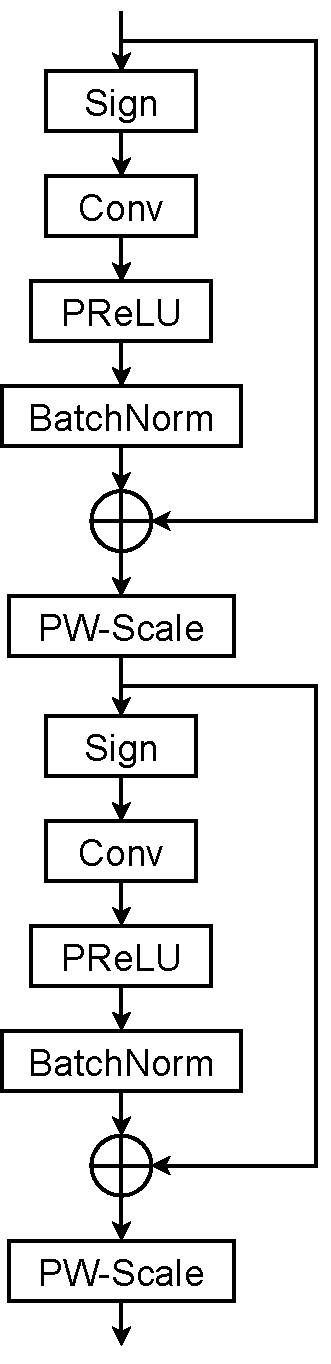
\includegraphics[width=0.22\textwidth]{pw.pdf}
  \caption{插入分段线性缩放函数的网络模块结构示意图}
  \label{fig:pw_block}
\end{figure}

为了最大化利用分段线性缩放模块的浮点计算能力,如图 \ref{fig:pw_block} 所示,本文将分段线性缩放函数插入到网络模块之间,使用该函数对浮点特征图进行调整。网络训练前,分段线性缩放函数的两个参数$\beta_1$和$\beta_2$均初始化为1,此时该函数等价于直通函数,训练过程中,参数$\beta_1$和$\beta_2$根据梯度自动进行优化,训练完成后分段线性缩放函数可以根据任务目标和网络结构自适应学习到合适的参数。

\section{实验分析}

为了验证本文设计的二值友好结构的性能,本文设计了如下实验:

1. 模块内网络层顺序对网络精度影响实验;

2. 模块间激活函数对网络精度影响实验。

模块内网络层顺序对网络精度影响实验探究了不同的网络层顺序与网络精度的关系,验证了本文提出的顺序最适合二值神经网络的训练。模块间激活函数对网络精度影响实验测试了多种不同模块间激活函数对二值网络性能的提升效果,验证了本文提出的分段线性缩放函数相比其他激活函数对二值网络的特征提取能力帮助更大。

\subsection{模块内网络层顺序对网络精度影响实验}

模块内网络层的排布顺序会显著影响二值神经网络的性能,目前为止提出的二值神经网络的网络层排布顺序几乎各不相同。本实验测试了多种模块内网络层排布方式,网络层的排布方式根据激活函数是否在残差连接内部分为两类,每类中有根据批归一化层的位置分为不同情况,本实验使用PReLU作为模块激活函数,激活函数在残差连接内部和外部的网络结构分别如图 \ref{fig:baseline1} 和图 \ref{fig:baseline2} 所示,其中数字表示可以插入批归一化层(BatchNorm)的位置,将在图 \ref{fig:baseline1} 中数字$x$处插入批归一化层的模块结构命名block1x,将在图 \ref{fig:baseline2} 中数字$x$处插入批归一化层的模块结构命名为block2x,所有网络进行二值网络的第一阶段训练结果如表 \ref{tab:42} 所示。

\begin{figure}[htbp]
  \vspace{6pt}
  \centering
  \begin{subfigure}{0.4\textwidth}
    \centering
    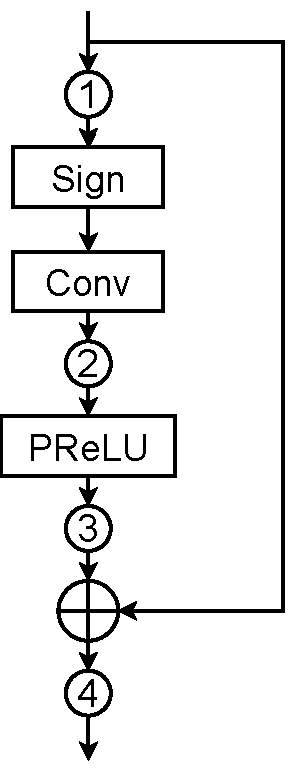
\includegraphics[width=0.55\textwidth]{baseline1.pdf}
    \caption{激活函数在残差连接内}
    \label{fig:baseline1}
  \end{subfigure}
  % \qquad
  \begin{subfigure}{0.4\textwidth}
    \centering
    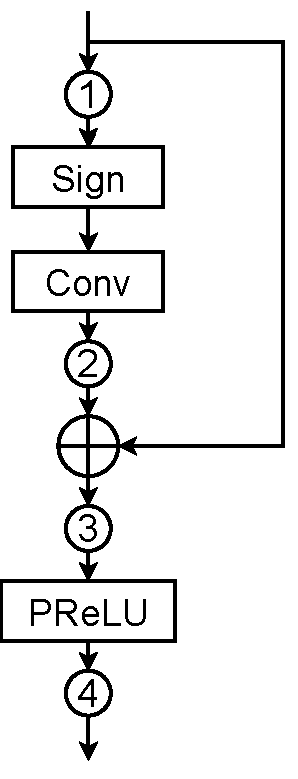
\includegraphics[width=0.55\textwidth]{baseline2.pdf}
    \caption{激活函数在残差连接外}
    \label{fig:baseline2}
  \end{subfigure}
  \caption{根据激活函数位置划分的两种网络层排布方法示意图}
  \label{fig:baseline}
  \vspace{6pt}
\end{figure}

\begin{table}[h]
  \vspace{6pt}
  \centering
  \caption{不同网络层排布顺序对网络精度影响表}
  \label{tab:42}
  \begin{tabular}{cc}
    \toprule
    模块结构 & Top-1精度(\%) \\
    \midrule
    block11 & 61.02 \\
    block12 & 61.46 \\
    block13 & \textbf{61.86} \\
    block14 & 61.08 \\
    block21 & 61.10 \\
    block22 & 60.32 \\
    block23 & 54.62 \\
    block24 & 58.83 \\
    \bottomrule
  \end{tabular}
  \vspace{6pt}
\end{table}

实验表明,PReLU激活函数在残差连接内部的模块结构精度普遍高于在外部的精度,表明符号函数不足以提供充足的非线性拟合能力,在卷积附近增加非线性激活函数可以增强网络的非线性能力,从而提高网络性能。所有实验结构中block13取得了最高的精度,该结构正是本文首次提出的将PReLU激活函数插入卷积层和批归一化层中间的模块结构。该结构精度最高表明PReLU激活函数与二值卷积组合使网络的特征提取能力得到了提升。

\subsection{模块间激活函数对网络精度影响实验}

\subsubsection{不同模块间激活函数对网络精度影响实验}

二值神经网络将激活值和权重二值化,使用二值卷积降低网络的计算量。与二值计算相比,浮点计算有更强大的特征解析能力,很多二值网络通过添加几乎忽略不计的浮点计算提升网络性能。本文提出在网络模块中间插入浮点激活函数层,以逐元素的方式对浮点特征图进行调整,调整方式由网络训练得到。本文使用分段线性缩放函数作为模块间的激活函数。本实验测试了多种模块间激活函数对第一阶段训练网络精度的影响,实验结果如表 \ref{tab:43} 所示。

\begin{table}[htb]
  \vspace{6pt}
  \centering
  \caption{不同模块间激活函数对网络精度影响表}
  \label{tab:43}
  \begin{tabular}{cc}
    \toprule
    模块间激活函数 & Top-1精度(\%) \\
    \midrule
    PReLU & 64.20 \\
    NPReLU & 64.06 \\
    RPReLU & 64.07 \\
    PW-Scale & \textbf{64.80} \\
    Scale & 64.15 \\
    \bottomrule
  \end{tabular}
  \vspace{6pt}
\end{table}

其中PReLU函数定义如公式 \eqref{eq:prelu} 所示。NPReLU函数定义如公式 \eqref{eq:nprelu} 所示。NPReLU函数与PReLU函数正好相反,正半轴具有可学习参数,负半轴保持输入不变。

\begin{equation}
  \label{eq:nprelu}
  f(x) =
  \begin{cases}
    \beta x & if \ x > 0 \\
    x & if \ x \leq 0
  \end{cases}
\end{equation}
RPReLU函数是ReActNet\cite{reactnet}网络中提出的激活函数,其函数定义如 \eqref{eq:rprelu} 所示。RPReLU函数在PReLU函数的基础上增加了两个可学习的偏移因子。

\begin{equation}
  \label{eq:rprelu}
  f(x) =
  \begin{cases}
    x - \gamma + \zeta  & if \ x > \gamma  \\
    \beta (x - \gamma) + \zeta  & if \ x \leq \gamma 
  \end{cases}
\end{equation}
PW-Scale函数是本文提出的分段线性缩放函数。Scale函数是单一的可学习缩放因子函数,定义如公式 \eqref{eq:scale} 所示,该缩放函数是线性函数。

\begin{equation}
  \label{eq:scale}
  f(x) = \beta x
\end{equation}

在上述所有激活函数方法中,本文提出的分段线性缩放函数取得了最高的网络精度。PReLU函数和NPReLU函数的精度相近,表明二值神经网络中正数特征和负数特征具有相同的价值。PW-Scale函数相比RPReLU少了两个浮点加法计算,但实验精度却比RPReLU函数高,证明了浮点特征缩放的效果好于浮点特征的偏移,使用训练得到的缩放系数对浮点特征进行缩放可以提高二值网络性能。

\subsubsection{有无模块间激活函数对网络精度影响实验}

为了进一步验证模块间分段线性缩放函数的效果,本文进行了模块间激活函数的消融实验。本文以不使用多特征图方法的Baseline-L和Baseline-H网络,使用多特征图方法的MFNet-S、MFNet-S和MFNet-L网络共5个网络结构为基础,分别测试了有模块间激活函数和无模块间激活函数的二值网络第一阶段训练精度。不同网络结构有计算量的区别,模块间激活函数使用本文提出的分段线性缩放函数,实验结果如表 \ref{tab:44} 所示。

\begin{table}[htb]
  \vspace{6pt}
  \centering
  \caption{有无模块间激活函数对网络精度影响表}
  \label{tab:44}
  \begin{tabular}{cccccc}
    \toprule
    网络结构 & \makecell{BOPs\\($\times10^9$)} & \makecell{FLOPs\\($\times10^8$)} & \makecell{OPs\\($\times10^8$)} & \makecell{无模块间激活函数\\Top-1精度(\%)} & \makecell{有模块间激活函数\\Top-1精度(\%)} \\
    \midrule
    Baseline-L & 4.58 & 0.12 & 0.84 & 68.44 & 69.15 \\
    Baseline-H & 8.79 & 0.12 & 1.49 & 69.68 & 70.05 \\
    MFNet-S    & 1.81 & 0.12 & 0.40 & 64.34 & 65.80 \\
    MFNet-B    & 3.09 & 0.12 & 0.60 & 67.22 & 68.63 \\
    MFNet-L    & 4.63 & 0.12 & 0.84 & 68.76 & 70.15 \\
    \bottomrule
  \end{tabular}
  \vspace{6pt}
\end{table}

可以看到,模块间插入分段线性缩放函数可以明显提升二值网络的推理精度。分段线性缩放函数可以将使用多特征图方法的网络精度提升1.5\%左右,将不使用多特征图方法的网络精度提升0.5\%左右。本文提出的分段线性缩放函数对多特征方法网络帮助更大,这是因为学习到的缩放因子$\beta$可以调整浮点特征的分布,浮点特征的分布直接影响不同阈值符号函数提取到的二值特征,网络通过优化缩放因子$\beta$可以得到更好的二值特征。

\section{本章小结}

在本章中,本文针对二值卷积的特点对网络结构进行了精心地设计,提出了二值友好的模块内网络层排布顺序。实验证明本文提出的网络层排布顺序在所有可能排布顺序中获得了最优的性能表现,验证了该二值友好结构的有效性。为了提高二值网络的特征提取能力,本文提出了模块间的分段线性缩放函数。实验验证该模块间激活函数可以有效提升二值神经网络的性能。